\documentclass[11pt,a4paper]{article}
\usepackage[margin=24mm]{geometry}
\usepackage[T1]{fontenc}\usepackage{lmodern,microtype}
\usepackage{amsmath,amssymb,amsthm,mathtools,bm}
\usepackage{booktabs,tabularx,graphicx,float,array,xcolor}
\usepackage[round,authoryear]{natbib}
\usepackage[colorlinks=true,allcolors=blue!55!black]{hyperref}
\newtheorem{theorem}{Theorem}[section]
\newtheorem{proposition}[theorem]{Proposition}
\newtheorem{corollary}[theorem]{Corollary}
\theoremstyle{remark}\newtheorem{remark}[theorem]{Remark}
\newcommand{\RR}{\mathbb R}\newcommand{\Prob}{\mathbb P}
\newcommand{\abs}[1]{\left|#1\right|}\newcommand{\norm}[1]{\left\|#1\right\|}
\newcommand{\boxx}{\mathcal X}\newcommand{\pp}{\mathcal P}
\title{\bfseries Reconstructed VQLS Corrections for AC Power Flow:\\ A Negative Certification Benchmark on IEEE 9- and 14-Bus Systems}
\author{Author names and affiliations to be confirmed}
\date{Revised research manuscript --- 2 November 2026}
\begin{document}\maketitle
\begin{abstract}
We assess single-step Newton corrections reconstructed from ideal-outcome, finite-shot variational quantum linear-solver (VQLS) simulations on IEEE 9- and 14-bus AC power-flow models. In eight fixed operating scenarios with three fixed training seeds each, we compare the same warm start against exact undamped one-step Newton, a residual-matched classical diagnostic, and converged Newton. An explicit importance-sampled Pauli estimator and signed-amplitude interference model establish what the simulator's 2.40--2.56 million ideal outcomes represent; the circuits were not executed and no hardware claims are made. Once the full correction is read out, an additional quantum residual estimate is redundant with classical evaluation. Likewise, the tested nonlinear root-inclusion contractor constructs a classical inverse-Jacobian preconditioner; the measured workflow does not avoid factorization. A second, separately written directed-rounding checker agrees with the 24 archived quantum inclusion decisions (3/12 on IEEE 9-bus and 0/12 on IEEE 14-bus) and establishes local enclosures for converged classical candidates in eight scenarios; this is not an external audit. Comparison with numerical reference roots separates three accepted 9-bus base candidates, three 14-bus base candidates lying within the largest tested boxes but failing inclusion, and 18 stressed candidates whose reference roots lie outside all tested candidate-centred boxes. Exact one-step Newton sharply reduces base-case errors; remaining stressed-case errors reflect both single-step nonlinearity and VQLS approximation. Only the three 9-bus base candidates undergo native-voltage and rated-branch screening under an extremely small parameter-uncertainty model; 14-bus results are root-inclusion tests only. The evidence supports an implementation-specific negative certification and feasibility benchmark, not a novel solver or a general quantum disadvantage theorem.
\end{abstract}
\noindent\textbf{Keywords:} Quantum power flow; variational quantum linear solver; negative feasibility benchmark; interval methods; classical readout; AC Newton correction; reproducibility.

\section{Introduction and research questions}
Quantum linear-system methods are useful when the required output consists of a limited number of quantum-state observables. A different problem arises in AC power flow: an operational Newton update requires the signed classical correction vector. This input/output distinction is central to quantum complexity claims \citep{hhl2009,aaronson2015,pareek2026}. Early quantum power-flow studies \citep{feng2021,feng2023} and recent VQLS applications \citep{feng2025,ninlawat2026} motivate testing complete reconstruction costs rather than solver loss alone.

Classical uncertainty and uniqueness methods for power flow have a long history \citep{wang1992,pereira2012,krawczyk1969,neumaier1990,rump2010}. Our purpose is not to reintroduce Krawczyk inclusion or a novel VQLS solver. We instead ask three falsifiable questions: (Q1) does an independently reconstructed finite-shot correction supply information unavailable by ordinary classical residual evaluation? (Q2) are certification and classical-preconditioner costs already sufficient to negate any savings in this implementation? (Q3) how much of poor acceptance is due to one Newton step from a distant warm start, rather than quantum approximation error? The resulting contribution is a \emph{reproducible negative feasibility benchmark} accompanied by candidate-specific interval checks and explicit diagnostic comparators.

The protocol evaluated here converts quantum amplitudes into a full classical vector and constructs a classical inverse-Jacobian preconditioner. Thus, unlike a hypothetical state-only output model, it has no asymptotic readout advantage to preserve; the precise failure mode is an empirical and algorithmic observation, not a claim of new mathematical impossibility for every quantum power-flow approach. The analysis is limited to steady-state equations under fixed PV/PQ classifications and small synthetic parameter intervals. IEEE 14-bus results are root-enclosure tests, not native security certificates.

\section{AC power-flow model and physical uncertainty}
Let $\mathcal G=(\mathcal V,\mathcal E)$ be a connected transmission network and $Y=G+\mathrm i B$ its bus-admittance matrix. For bus $i$ with voltage magnitude $v_i$ and angle $\theta_i$,
\begin{align}
P_i(x;p)&=\sum_{j=1}^n v_i v_j\bigl(G_{ij}(p)\cos(\theta_i-\theta_j)+B_{ij}(p)\sin(\theta_i-\theta_j)\bigr),\\
Q_i(x;p)&=\sum_{j=1}^n v_i v_j\bigl(G_{ij}(p)\sin(\theta_i-\theta_j)-B_{ij}(p)\cos(\theta_i-\theta_j)\bigr).
\end{align}
Eliminating the slack-bus angle and treating PV-bus voltages as prescribed produces $F_p(x)=0$ on $d=n_{\mathrm{PV}}+2n_{\mathrm{PQ}}$ coordinates. This study holds the bus-type assignment fixed; generator reactive-limit switching and dynamic or transient stability are \emph{not} certified.

The parameter box $\pp$ comprises admissible primitive line resistances $r_\ell$, reactances $x_\ell$, charging susceptances $b_\ell$, applicable tap ratios $\tau_\ell$, and specified injections. Uncertainty must be propagated through $y_\ell=(r_\ell+\mathrm i x_\ell)^{-1}$ and the bus-admittance construction, rather than perturbing its entries independently. A branch outage changes network topology and requires rebuilding $F_p$ and its Jacobian. Tests assume non-islanding and a fixed reference convention; islanded scenarios require another model.

For an initial operating state $x_0$ let $A=J_{p_0}(x_0)$ and $b=-F_{p_0}(x_0)$; the ideal Newton correction obeys $Az=b$. A trial correction $\widehat z$ creates the \emph{actual applied centre} $\widehat x=x_0+\widehat z$.

\section{What is measured, reconstructed, and checked?}\label{sec:readout}
\subsection{Experimental operator and ideal-outcome sampling protocol}
The final 24-run archive uses the \emph{direct padded nonsymmetric Jacobian}, not the earlier Hermitian embedding. Write $A=J_{p_0}(x_0)\in\mathbb R^{d\times d}$, $p=2^q\ge d$, $\widetilde A=\mathrm{diag}(A,0_{p-d})$, $M=\widetilde A/\|A\|_2$, $K=M^\dagger M$, and $u=(b/\|b\|_2,0_{p-d})$. The normalized real-amplitude tree ansatz $v(\theta)=U_\theta|0^q\rangle$ has $p-1$ trainable rotation angles. With $M=\sum_{\ell}c_\ell P_\ell$ and $K=\sum_j d_jP_j$, the trace-rule coefficients $c_\ell=2^{-q}\operatorname{tr}(P_\ell M)$ may be complex (the nonsymmetric $A$ has odd-$Y$ terms), while $d_j$ are real up to roundoff because $K$ is Hermitian. No imaginary term is discarded. The numerator uses respectively 200 and 864 nonzero $M$ terms (88 and 416 with nonzero imaginary part); the denominator uses respectively 136 and 528 nonzero $K$ terms.

Define $\Gamma_M=\sum_\ell|c_\ell|$, $\Gamma_K=\sum_j|d_j|$ and select independent term indices $L\sim|c_\ell|/\Gamma_M$ or $J\sim|d_j|/\Gamma_K$. Conditional on $L=\ell$, an ideal phase-adjusted Hadamard overlap test prepares
\begin{equation}\label{eq:overlapcircuit}
\frac{|0\rangle|u\rangle+|1\rangle e^{\mathrm i\arg c_\ell}P_\ell|v\rangle}{\sqrt2},\qquad
\mathbb E[H_\ell\mid L=\ell]=\operatorname{Re}\!\left[e^{\mathrm i\arg c_\ell}\langle u|P_\ell|v\rangle\right]
\end{equation}
by measuring ancilla $X$, with $H_\ell\in\{-1,+1\}$. A numerator shot is $Z_a=\Gamma_M H_L$. For the denominator, a Pauli measurement on $|v\rangle$ gives $Q_J\in\{-1,+1\}$ and a shot is $Z_D=\Gamma_K\operatorname{sgn}(d_J)Q_J$. These choices correspond to the \emph{separately and classically assembled} $K=M^\dagger M$, not term-pair sampling. The exact ideal distribution has
\begin{align}\label{eq:unbiased}
\mathbb E Z_a&=a:=\operatorname{Re}\langle u|Mv\rangle,&\operatorname{Var}(Z_a)&=\Gamma_M^2-a^2,\\
\mathbb E Z_D&=D:=\langle v|Kv\rangle,&\operatorname{Var}(Z_D)&=\Gamma_K^2-D^2.
\end{align}
Hence each empirical mean based on $N$ independent outcomes has variance $\operatorname{Var}(Z)/N$ and $|Z_a|\le\Gamma_M$, $|Z_D|\le\Gamma_K$. Equation~\eqref{eq:unbiased} is an estimator specification, not a claim of improved shot complexity. The implementation samples multinomial term counts and binomial signs directly from the analytical Born probabilities, without executing the controlled preparation gates. The input construction of $u$, $M$, and $K$ is classical and should be included in any end-to-end cost ledger.

\paragraph{Signed coordinate measurement and phase convention.} Each physical coordinate $i<d$ is sampled independently with a separate ancilla test preparing $(|0\rangle|i\rangle+|1\rangle|v\rangle)/\sqrt2$. Its $X$ outcome $H_i\in\{\pm1\}$ obeys $\mathbb E H_i=\operatorname{Re}\langle i|v\rangle=v_i$ for the real tree ansatz. Thus $\widehat v_i=2B_i/N_i-1$ for $B_i\sim\operatorname{Binomial}(N_i,(1+v_i)/2)$, $\operatorname{Var}(\widehat v_i)=(1-v_i^2)/N_i$. This measures \emph{signed interference}, not $|v_i|^2$. It requires coherent controlled $U_\theta$ and a specified relative phase between the $|i\rangle$ and $|v\rangle$ preparations. The same circuit-level phase convention is used for the signed numerator overlap $a$; global phase is therefore fixed only relative to these coherent preparation controls, not by computational-basis probabilities. In the archived simulation the ideal circuit amplitudes determine \emph{sampling probabilities}, not the output estimates; no signed amplitude is copied directly into the reconstructed correction. The padded coordinates $i\ge d$ are not read out, physical estimates are \emph{not renormalized}, and different $i$ use disjoint binomial draws. The unmeasured padded component remains part of the normalized training state and can reduce physical correction norm.

\paragraph{Training and holdout scale safeguards.} The sampled training objective is the global projective cost
\begin{equation}\label{eq:traincost}
 \widehat L(\theta)=1-\frac{\widehat a(\theta)^2}{\max\{\widehat D(\theta),0.08\}},\qquad
 L(\theta)=1-\frac{a(\theta)^2}{D(\theta)}.
\end{equation}
The clipping at $0.08$ applies \emph{only during training}. The archived holdout code computes
\begin{equation}\label{eq:zreconstruct}
 \widehat s=\frac{\|b\|_2}{\|A\|_2}\frac{\widehat a}{\widehat D},\qquad \widehat z=\widehat s\widehat v_{1:d},\qquad \widehat x=x_0+\widehat z,
\end{equation}
if $\widehat D>0$, and returns an undefined scale (NaN) otherwise; it does \emph{not} silently use the training clip. All 24 archived holdouts were flagged as allowing a positive-denominator confidence interval. For an executable deployment the acceptance policy must \emph{reject/abstain} if $\widehat D\le0$, if a simultaneously valid lower confidence limit for $D$ is nonpositive when interval scale control is required, or if any reconstructed value is nonfinite. No near-zero-denominator stability guarantee is claimed for the original training code. The supplemental algorithm specifies the original record and this prospective safe-abstention policy separately.

\begin{figure}[htbp]\centering
\fbox{\begin{minipage}{.91\linewidth}\small\textbf{Algorithm 1 (ideal-outcome, fixed-seed record).} Given $A,b,\theta$, decompose $M$ and the classically formed $K=M^\dagger M$. At each SPSA cost call, independently draw 4000 outcomes of $Z_a$ and 4000 of $Z_D$, then use Eq.~\eqref{eq:traincost}. After 120 updates, estimate $a$ and $D$ using 100000 fresh outcomes each. Draw 10000 signed interference outcomes \emph{per physical coordinate} to construct $\widehat v$. The archived study also draws 10000 extra Pauli-residual outcomes per coordinate (redundant after reconstruction). Reconstruct $\widehat z$ by Eq.~\eqref{eq:zreconstruct} when defined; compute $A\widehat z-b$ classically and apply the separate interval checker. All random outcomes in the archived execution are simulated from ideal probabilities, not circuit outputs.\end{minipage}}
\caption{Operational specification and shot ledger for the archived sampling abstraction. The indicated conditional circuits are mathematical realizations of each outcome, not circuits executed in this study.}\label{fig:oraclealgorithm}
\end{figure}

\subsection{Residual redundancy and the appropriate physical check}
Because $A$, $b$ and $\widehat z$ are all classically available, the directly computed residual
\begin{equation}\label{eq:exactresidual}
 r_{\rm cl}=A\widehat z-b
\end{equation}
requires only $O(\operatorname{nnz}(A))$ arithmetic after matrix construction, apart from ordinary floating-point roundoff. If rigorous enclosures are desired, the interval contractor can evaluate $F_p(\widehat x)$ directly. A Hoeffding bound on a second quantum estimate of $A\widehat z-b$ adds width but supplies no independent physical information for the present output model. We therefore \emph{remove quantum residual measurements from the claimed certification contributions}. Those additional holdout shots are retained in the experimental resource ledger as wasted verification cost.

The exact classical mismatch at a nominal parameter value may be estimated as $F_{p_0}(\widehat x)$, while the parameter-uniform mismatch is enclosed by evaluating $F_p(\widehat x)$ over $p\in\mathcal P$ with directed interval arithmetic. For comparison with earlier analytic bounds, Taylor's theorem gives
\begin{equation}\label{eq:mismatch}
 |F_p(x_0+\widehat z)|_i\le |r_{\rm cl}|_i+\delta_{F,i}+\sum_jD_{J,ij}|\widehat z_j|+\tfrac12\sum_{jk}M_{ijk}|\widehat z_j\widehat z_k|,
\end{equation}
provided the specified first- and second-derivative majorants hold over the whole correction segment. The numeric contractor in this paper directly encloses $F_p(\widehat x)$; it does not need the finite-shot residual bound. A \emph{state-only} algorithm that never reads out the correction could use quantum observables, but constructing a compatible nonlinear enclosure without full readout is a different, untested research problem \citep{li2026}.

\section{Nonlinear parameter-uniform certification}\label{sec:cert}
Fix a candidate box $\boxx=\{x:|x-\widehat x|\le \bar t\}$ with a positive vector $\bar t$, and a fixed nonsingular preconditioner $B_0$. Assume $F_p$ is continuously differentiable on an open neighbourhood of $\boxx$, uniformly for the considered $p\in\pp$. Suppose an outwardly bounded matrix $C\ge0$ satisfies
\begin{equation}\label{eq:C}
|I-B_0J_p(x)|\le C\quad(x,p)\in\boxx\times\pp.
\end{equation}
For every $p$ write $T_p(x)=x-B_0F_p(x)$. The following statement ensures a root enclosure, not necessarily a complete physical security certificate.
\begin{theorem}[Candidate-source-independent root and security enclosure]\label{thm:root}
Assume \eqref{eq:C}. If a nonnegative vector $u$ bounds $|F_p(\widehat x)|$ for all $p\in\pp$ (for example by direct interval evaluation) and
\begin{equation}\label{eq:inclusion}
|B_0|u+C\bar t<\bar t\qquad\text{componentwise},
\end{equation}
then $\forall p\in\pp\;\exists!\,x_p^*\in\boxx$ such that $F_p(x_p^*)=0$; no claim of global uniqueness outside $\boxx$ follows. This implication remains valid when the centre is a random quantum-trained and reconstructed state, provided the centre and numerical enclosure $u$ are valid. If a physical signed constraint $s_j(x;p)\le0$ has validated centre approximation $\widehat q_j$, validated allowance $D_j$ for centre-evaluation and parameter variation at the centre and gradient majorant $g_j\ge0$ on $\boxx\times\pp$, then
\begin{equation}\label{eq:margin}
s_j(x_p^*;p)\in[\widehat q_j-W_j,\widehat q_j+W_j],\quad W_j=D_j+g_j^\mathsf T\bar t.
\end{equation}
In particular, a nonpositive upper endpoint certifies satisfaction, a strictly positive lower endpoint certifies violation, and all other cases are indeterminate.
\end{theorem}
\begin{proof}
For any $x\in\boxx$, the integral mean-value formula along the segment between $\widehat x$ and $x$ and \eqref{eq:C} yield
$|T_p(x)-\widehat x|\le|B_0F_p(\widehat x)|+C|x-\widehat x|<\bar t$.
The map therefore carries $\boxx$ into itself. Because $\bar t>0$ and $|B_0|u+C\bar t<\bar t$, we have $C\bar t<\bar t$; the Collatz--Wielandt bound gives $\rho(C)\le\max_i(C\bar t)_i/\bar t_i<1$. The weighted maximum norm associated with $\bar t$ therefore makes $T_p$ a strict contraction on $\boxx$. Banach's fixed-point theorem gives exactly one fixed point there for each $p$. Nonsingularity of $B_0$ makes it a root of $F_p$. Integrating the gradient bound from $\widehat x$ to the root, and adding the validated centre/parameter allowance, gives \eqref{eq:margin}.
\end{proof}
\begin{remark}
The existence-and-uniqueness argument is standard contraction/Krawczyk theory. The theorem is exact \emph{conditionally on valid enclosures}; it is not a retrospective guarantee that the archived computations met its hypotheses. To claim a formally machine-verified numerical certificate, every input decimal, interval trigonometric operation, matrix product, nonnegative majorant, and strict endpoint comparison must be enclosed with independently checked outward rounding. The archival implementation alone has not passed such an audit. Section~\ref{sec:secondverification} reports complete 24-flag corroboration by a separate directed-decimal implementation, but no third-party audit has been performed \citep{krawczyk1969,moore1966,neumaier1990,rump2010}.
\end{remark}

\subsection{Sharper a posteriori enclosure}
For a given centre let $d_0\ge|B_0F_p(\widehat x)|$ for all $p\in\mathcal P$ and suppose $C$ is an entrywise nonnegative, validated uniform Jacobian majorant satisfying the strict box test. Then the nonnegative comparison matrix has $\rho(C)<1$, and the \emph{sharper} fixed-point radius
\begin{equation}\label{eq:H}
 t=(I-C)^{-1}d_0\le\bar t
\end{equation}
bounds $|x_p^*-\widehat x|$ componentwise, provided $C$ has been validated on the original containing box $\boxx$. Thus $D_j+g_j^\mathsf T t$ may replace the coarser observable allowance $D_j+g_j^\mathsf T\bar t$. The displayed numerical study reports the original verified boxes, not a newly recalculated table of tightened observable widths. Floating-point matrix inversion is not itself a validated computation of this bound.

\section{Computed preconditioner, validated arithmetic and classical cost}\label{sec:precond}
The evaluated contractor forms the binary floating-point matrix
\begin{equation}\label{eq:preconditioner}
B_0=\operatorname{fl}\!\left(J_{p_0}(\widehat x)^{-1}\right)
\end{equation}
by dense numerical inversion at the \emph{reconstructed candidate centre}, not at the warm start $x_0$. The theorem needs a fixed nonsingular $B_0$ for which $|I-B_0J_p(x)|$ is enclosed on the box; it neither requires $B_0$ to equal the exact inverse nor requires an interval matrix enclosing the exact inverse. One may treat each stored binary number in $B_0$ as \emph{exactly represented} and use directed arithmetic when importing and multiplying those entries. The approximation error relative to the mathematical inverse is already represented by the certified $I-B_0J$ defect. No exact inverse containment assertion is made. A strict $\|I-B_0J\|_w<1$ for a nonsingular nominal $J$ also implies $B_0$ is nonsingular. The independent checker imports $B_0$ using exact binary-to-decimal conversion and bounds the subsequent matrix products and strict comparisons; it does not certify the exactness of the numerical factorization.

Computing $B_0$ nevertheless performs a classical Jacobian factorization sufficient to support a further classical Newton update $\Delta x=-B_0F_{p_0}(\widehat x)$ (up to the inverse approximation). This is \emph{not} the same step as the exact one-step comparator from $x_0$, and their end-to-end iteration counts and certification-call counts may differ. The implemented workflow does not avoid classical Jacobian factorization: it adds quantum training and reconstruction before a certification stage that already computes a factorization suitable for Newton refinement. \emph{The reported experiments provide no evidence of an end-to-end benefit.} No general lower bound forbidding savings for other candidate quality, certification methods, iterations or quantum architectures is asserted.

Once the entire correction is reconstructed, a new quantum measurement of $A\widehat z-b$ is informationally redundant; it can be computed classically in $O(\operatorname{nnz}A)$ arithmetic, or enclosed with verified floating-point arithmetic. The archived residual-oracle shots are retained in resource accounting only. We do not claim a new general stopping or shot-allocation theorem for this reconstructed-output design.

\section{Experimental protocol and fixed-seed provenance}\label{sec:method}
The MATPOWER \texttt{case9} and \texttt{case14} data provide reduced Newton systems of dimensions $d=14$ and $d=22$ \citep{zimmerman2011,matpowercase9,matpowercase14}. Eight operating conditions are tested: intact base case, $20\%$ proportional increase in active/reactive demands, one specified N--1 branch outage, and a $10\%$ load increase together with another N--1 outage, separately for each network. PV/PQ bus types and generator active-power setpoints remain fixed. Each scenario begins at an identical favourably initialized base-case solution plus a deterministic $0.0012\sin(0.73j+0.5)$ state perturbation; no scenario-specific operating-point convergence is fed into the VQLS training.

For each condition, seeds $711$, $713$ and $717$ generate fixed ideal-outcome simulated readouts. The real-amplitude tree ansatz uses $15$ and $31$ parameters respectively, with logical state-preparation depth $4$ and $5$ rotation levels (no compiled device depth). The SPSA schedule has $120$ iterations, two noisy objective evaluations per iteration, Rademacher perturbations, and $c_k=0.20k^{-0.101}$, $a_k=0.055(k+12)^{-0.602}$ with componentwise gradient clipping at $\pm6$. The sampled objective uses $4000$ shots each for $a$ and $D$, per evaluation, or $1.92\times10^6$ training outcomes per run. The holdout uses $100000$ shots each for scale numerator and denominator, plus $10000$ shots \emph{per physical coordinate} for amplitude reconstruction and another $10000$ per coordinate for an auxiliary quantum-residual estimate that is \emph{redundant after readout}. The totals are $2.40\times10^6$ (9-bus) and $2.56\times10^6$ (14-bus). These are \emph{simulated ideal Pauli outcomes}, not Qiskit-Aer circuits, hardware shots, calibrated noise tests or a physical device gate-level cost. The sampling implementation computes the conditional Born probabilities from an exact NumPy statevector solely to simulate ideal outcomes; this probability oracle is not evidence that a real circuit estimates the same quantities at the counted gate cost. The independently produced supplemental sampler check verifies unbiasedness against those ideal probabilities in a fresh Monte Carlo test, not gate-level implementation. An ideal projective loss is recomputed only \emph{after training} for diagnostic reporting; it is not supplied to the optimizer.

For each fixed seed and scenario we compare: (i) the read-out VQLS $\widehat z$; (ii) the exact classical single Newton correction $z_N=A^{-1}b$ from the \emph{same} $x_0$; (iii) a \emph{diagnostic} residual-matched classical correction $z_{\rm M}=(1-\lambda)z_N$, where $\lambda=\min\{1,\|A\widehat z-b\|_\infty/\|b\|_\infty\}$; and (iv) a separately iterated classical Newton solution from the same $x_0$. Since $Az_N=b$, $\|Az_{\rm M}-b\|_\infty=\lambda\|b\|_\infty$, which equals the VQLS residual when it does not exceed $\|b\|_\infty$. The damped LU solution already pays for a complete factorization; it is a \emph{diagnostic control}, neither an accuracy-matched nor cost-matched competing solver. In the archived 24 VQLS trials the target residual exceeded $\|b\|_\infty$ in 0 trials, so clipping did not prevent exact infinity-norm matching in this fixed data set. Reference roots $x^*$ are computed classically solely to diagnose state errors, not to train the quantum correction.

We report $\|x_0-x^*\|_\infty$, $\|x_0+z-x^*\|_\infty$, $\|z-z_N\|_2/\|z_N\|_2$, $\|Az-b\|_\infty$ and $\kappa_2(A)$. The additional left-singular residual projection $\|\Pi_{\rm small}U^\mathsf Tr\|_2^2/\|r\|_2^2$ characterizes which residual directions are amplified by the inverse; the plotted state-error differences are not attributed to quantum noise alone.

\paragraph{Intervals and physical scope.} Let $\delta=10^{-7}$ denote the \emph{relative} half-width for each nonzero primitive resistance, reactance, charging or applicable tap input: $a\in[a_0-|a_0|\delta,a_0+|a_0|\delta]$. Independently, every specified injection/mismatch component has an \emph{absolute} uncertainty half-width $0.01\delta=10^{-9}$ p.u. This is not a one-per-cent demand change; the scenario load multipliers are separate deterministic modifications. The primary acceptance radii are $\{0.0015,0.003,0.006\}$ on 9-bus and $\{0.0025,0.005,0.010\}$ on 14-bus. Larger tested relative primitive uncertainties $10^{-4}$--$10^{-3}$ did not obtain inclusion even for classical root-centred checks in the original contractor, so no realistic-uncertainty capability is claimed. We have \emph{not} isolated the interval dependency/contractor failure mechanism, and omit ``parameter-uniform at meaningful uncertainty'' from the contribution list. Exact input decimals and fixed seeds are included in the available local reproducibility files; a public DOI has not been created.

\section{Results: single-step bias, error direction and inclusion}\label{sec:results}
\begin{table}[htbp]\centering\scriptsize\setlength{\tabcolsep}{4pt}
\caption{\textbf{New diagnostic comparison from the archived fixed seeds.} State errors are infinity norms relative to a separately converged nominal reference root $x^*$; VQLS and matched-LU entries are medians of three fixed seeds. Exact single-step Newton is deterministic. These state distances are diagnostic point values, \emph{not} interval guarantees. Network 14 is assessed only for root proximity.}
\begin{tabular}{@{}llrrrrr@{}}\toprule
Bus & Condition & $\kappa_2(A)$ & $\|x_0-x^*\|_\infty$ & VQLS error & Matched-LU error & Newton-step error \\\midrule
9 & Base & 58.3 & 0.0012 & 0.00087 & 0.00043 & 5.5e-06 \\
9 & Load $+20\%$ & 58.3 & 0.086 & 0.082 & 0.048 & 0.0018 \\
9 & Outage 4--5 & 125.9 & 0.19 & 0.18 & 0.15 & 0.012 \\
9 & Load/outage & 131.4 & 0.47 & 0.45 & 0.38 & 0.084 \\
14 & Base & 117.6 & 0.0012 & 0.0012 & 0.00038 & 1e-05 \\
14 & Load $+20\%$ & 117.6 & 0.064 & 0.063 & 0.053 & 0.0008 \\
14 & Outage 1--2 & 250.8 & 0.55 & 0.51 & 0.24 & 0.084 \\
14 & Load/outage & 198.4 & 0.29 & 0.28 & 0.15 & 0.018 \\
\bottomrule\end{tabular}\label{tab:errors}\end{table}
\begin{figure}[htbp]\centering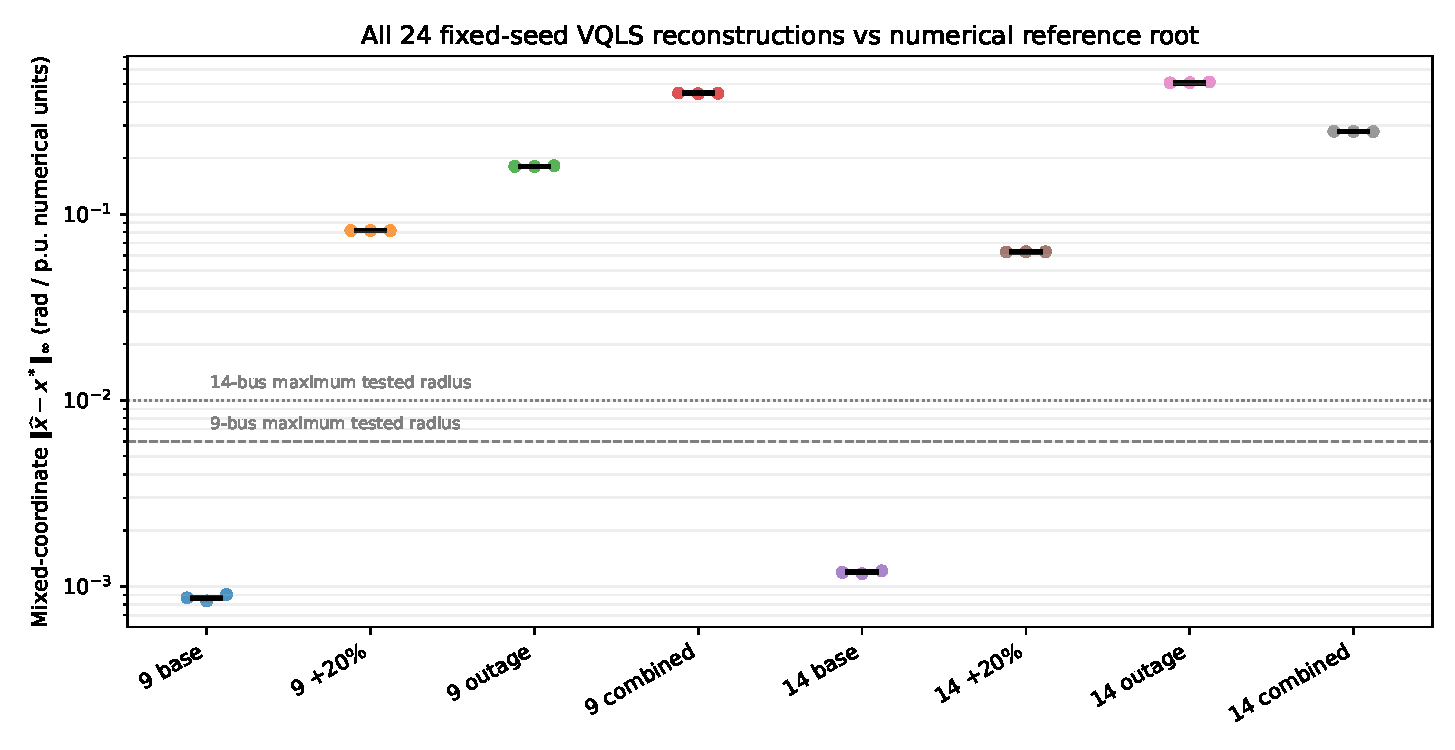
\includegraphics[width=\linewidth]{all_seed_root_distances.pdf}
\caption{All 24 fixed-seed reconstructed VQLS candidates plotted individually against the separately computed numerical nominal reference root. Short black bars show within-scenario medians; dashed horizontal levels indicate the largest tested box radii for the respective networks. The vertical axis is a mixed-coordinate numerical infinity norm (angles in radians, PQ magnitudes in p.u.), not a dimensionless physical metric or an interval enclosure. No additional training was performed.}\label{fig:distance}\end{figure}
\begin{table}[htbp]\centering\small
\caption{Candidate-centred \emph{root-inclusion} flags at $\delta=10^{-7}$, confirmed by a separately implemented directed-decimal checker for VQLS and iterated Newton, but not externally audited. Matched-LU and exact-one-step flags are archival interval-contractor results and are \emph{not} separately cross-checked in this revision. VQLS and matched LU have three fixed seeds; exact one-step Newton is one deterministic trial. IEEE 14-bus entries are \emph{not security certificates}.}
\begin{tabular}{@{}llccc@{}}\toprule
Bus & Condition & VQLS & Matched LU & Exact single step \\\midrule
9 & Base & 3/3 & 3/3 & Pass \\
9 & Load $+20\%$ & 0/3 & 0/3 & Fail \\
9 & Outage 4--5 & 0/3 & 0/3 & Fail \\
9 & Load/outage & 0/3 & 0/3 & Fail \\
14 & Base & 0/3 & 3/3 & Pass \\
14 & Load $+20\%$ & 0/3 & 0/3 & Fail \\
14 & Outage 1--2 & 0/3 & 0/3 & Fail \\
14 & Load/outage & 0/3 & 0/3 & Fail \\
\bottomrule\end{tabular}\label{tab:flags}\end{table}

\paragraph{Separation of solver and one-step errors.} A correct Newton step is not a converged nonlinear solution. In the 9-bus outage case the warm-start distance is approximately $0.191$, and one exact Newton step still leaves $0.0119$ infinity-norm state error. In the 14-bus outage of line 1--2, the corresponding distances are $0.551$ and $0.0839$. Thus failure of the one-step inclusion sweep in stressed cases cannot be attributed exclusively to finite-shot sampling. Conversely, in the base cases, the exact single step leaves only $5.5\times10^{-6}$ (9-bus) and $1.03\times10^{-5}$ (14-bus) error, while VQLS medians remain $8.68\times10^{-4}$ and $1.19\times10^{-3}$. The sampled quantum approximation is independently consequential there.

\paragraph{Equal residual magnitudes do not imply equal state errors.} For IEEE 14-bus base the residual-matched LU has the same infinity-norm residual as VQLS by construction (median $\approx0.0102$ p.u.), yet the median state errors are $3.83\times10^{-4}$ and $1.19\times10^{-3}$, respectively. Since $z-z_N=A^{-1}(Az-b)$, residual orientation relative to the left singular vectors of $A$ directly changes correction error. The 14-bus base Jacobian has $\kappa_2(A)\approx117.6$ versus $58.3$ for 9-bus base. Across the 14-bus base VQLS seeds, the median relative correction error $\|\widehat z-z_N\|_2/\|z_N\|_2$ is $0.800$, compared with $0.314$ for the matched LU corrections. These observations support a \emph{direction-sensitive} interpretation, not a universal explanation of every failed certificate. Detailed seed-level residuals and projections are in \path{diagnostics.csv}.

\subsection{Reference-root geometry and fixed-radius non-certification}
Every candidate was compared with the \emph{numerically computed nominal reference root} $x^*$ using the largest tested box radius $r_{\max}=0.006$ for IEEE 9-bus and $0.010$ for IEEE 14-bus. This is a diagnostic classification: a numerical reference root outside a box does not prove that \emph{no other} root exists inside it. The 24 trials decompose as follows.
\begin{table}[htbp]\centering\small
\caption{Mutually exclusive diagnoses across the 24 fixed-seed VQLS candidates. ``Outside'' refers solely to the separately computed nominal reference root; ``no inclusion'' is failure of a sufficient test, never proof of absence of a solution.}
\begin{tabular}{@{}lrrr@{}}\toprule
Network & Included & Ref. root beyond $r_{\max}$ & Ref. inside, no inclusion \\\midrule
IEEE 9-bus (12 trials) & 3 & 9 & 0 \\
IEEE 14-bus (12 trials) & 0 & 9 & 3 \\
Total & 3 & 18 & 3 \\\bottomrule
\end{tabular}\label{tab:geometry}
\end{table}
The three 14-bus base cases demonstrate the distinction most clearly: the nominal reference root lies within the largest candidate-centred box, but the chosen interval majorant does not establish strict inclusion. In all 18 stressed trials the numerical reference root is beyond the largest box, consistent with poor candidate placement and single-step warm-start limitations. Each raw seed and reference-root distance is supplied in \path{trial_level_geometry.csv}. The gap does not establish that the contractor alone caused all the 14-bus failures.

\paragraph{Uncertainty generality.} The nominal-root results above should not be confused with a solution under operationally representative parameter intervals: all positive parameter-uniform inclusions in the table use $\delta=10^{-7}$, an extraordinarily small primitive interval. The unsuccessful larger-$\delta$ runs did not separately diagnose whether parameter shifts, interval dependency or box selection caused failure; we therefore do not extrapolate the parameter-uniform method's effectiveness beyond those targets.

\section{Physical security scope and resource feasibility}\label{sec:security}
\subsection{Root inclusion is not a security decision}
A root-inclusion flag establishes only the local existence/uniqueness predicate in Theorem~\ref{thm:root}, and only provisionally for the present numerical outputs. Physical security requires an \emph{additional} outwardly enclosed check of each relevant bus-voltage bound and rated branch-flow constraint over \emph{every} state and parameter in the computed box. The scope of the numerical evidence is therefore:
\begin{itemize}\setlength{\itemsep}{2pt}
\item \textbf{IEEE 9-bus, intact base case:} the three quantum-produced corrections with positive provisional root-inclusion flags also had positive provisional native bus-voltage ($0.9$--$1.1$ p.u.) and rated-branch apparent-power screenings at the very small tested uncertainty levels. These are the \emph{only} quantum-derived cases in the final stress study for which a native steady-state security check was reported as passed, and even they are not independently verified proofs.
\item \textbf{IEEE 9-bus, stressed cases:} no quantum candidate passed the chosen root-inclusion sweep. Classical candidates sometimes admit provisional root enclosures without complying with all native operating limits; in particular, the archived combined load/outage case fails a native voltage screen. Neither a provisional root inclusion nor a failed inclusion is a blanket security verdict.
\item \textbf{IEEE 14-bus, all four scenarios:} \textbf{root-inclusion feasibility only.} MATPOWER \texttt{case14} has zero/unspecified branch MVA ratings and fixed generator voltage setpoints $1.07$ and $1.09$ p.u. at buses 6 and 8, above the native $1.06$-p.u. upper bus limit \citep{matpowercase14}. Thus we do not certify compliance with that benchmark's full native operating limits, even for classical corrections whose root-inclusion tests pass. A $0.9$--$1.1$-p.u. illustrative screen is not a substitute for native limits.
\end{itemize}
We claim neither transient stability nor reactive-limit security; PV/PQ switching, generator reactive limits and contingency redispatch are outside the validated model.

\subsection{Structural and measured resource comparisons}
The expense is not merely the number of simulated shots. Under the tested implementation, the classical output already consists of all $d$ signed amplitudes, the matrix $A$ and right-hand side $b$ are stored classically, and $B_0=J_{p_0}(\widehat x)^{-1}$ is formed by a dense inverse before the Krawczyk test. The same factorization could support a classical Newton refinement, but the cost of this candidate-centred calculation is not identical to the warm-start comparator and a universal runtime impossibility does not follow. The added ideal-outcome training, signed readout and redundant residual measurements are uncompetitive in the observed small-system comparison. A state-only, no-readout solver with another certification mechanism would be a different algorithm.

For descriptive resource illustration only, $2.40\times10^6$ and $2.56\times10^6$ ideal outcome samples were drawn per fixed-seed run. Prior Python/SciPy sparse-LU factor-and-solve medians were $62$ and $71\,\mu$s for $14\times14$ and $22\times22$ matrices, respectively. These tiny times are subject to substantial Python call, object construction and sparse-factorization overhead and are \emph{not} hardware-neutral compute kernels; processor model, exact dependency versions and CPU affinity were not preserved with those historical medians. At an explicitly \emph{unphysically optimistic} $1$ ns per result, ideal sampling alone requires $2.40$--$2.56$ ms, roughly 39 and 36 times the measured LU medians; the implied simplistic per-shot parity targets of 26 and 28 ps ignore other quantum costs. Actual device timings would include state preparation, compiled controlled gates, readout/reset, noise mitigation, queueing, full signed-amplitude reconstruction and classical inverse construction. None are benchmarked, so we make no hardware runtime or speedup claim. The precise structural finding is that full readout and candidate-centred classical inversion remove the \emph{claimed avoided factorization} in this implementation; the data do not imply a hardware-independent theorem about every end-to-end solver.

\section{Separate-implementation numerical cross-check}\label{sec:secondverification}
\begin{table}[htbp]\centering\scriptsize
\caption{Independence boundary of the second checker. An independently written arithmetic kernel does not make the entire numerical evidence independent.}
\begin{tabularx}{\linewidth}{@{}p{34mm}X@{}}\toprule
Component & Relationship between original and second checker \\\midrule
Scenario inputs and decimals & Same benchmark numerical inputs and outage specifications; second checker parses source decimal tokens directly rather than first rounding them to binary floats. \\
Candidate corrections & Shared/replayed fixed-seed VQLS outputs and warm-start protocol; not independently generated training data. \\
Admittance assembly & Separately coded from the same primitive branch model and identical physical assumptions. \\
Power flow / Jacobian & Separately coded interval equations and interval Jacobian; both share coordinate ordering and PV/PQ conventions. \\
Transcendental intervals & Original \texttt{mpmath.iv}; second exact-rational Taylor remainder plus directed-\texttt{Decimal} arithmetic. \\
Preconditioner & Same classically computed floating inverse at each candidate; second checker imports its binary entries as exact numbers. \\
Test radii / acceptance & Same predetermined radius list; independent strict endpoint comparisons. \\
Voltage / branch screens & Independently coded IEEE 9-bus directed-interval screening, sharing the same native limits and rated branch data; no complete native 14-bus screen. \\\bottomrule
\end{tabularx}\label{tab:independence}
\end{table}
Agreement on the three \emph{positive} VQLS inclusions provides distinct evidence from agreement on the 21 \emph{failed sufficient tests}. A negative flag is not an independently verified root-exclusion theorem, and an external audit has not been performed.

To test the reliability of the archived \texttt{mpmath.iv} verdicts without relying on their float-converted interval endpoints, we independently implemented a second Krawczyk checker in Python. It parses literal input decimals into directed \texttt{Decimal} intervals (65-digit arithmetic), uses exact-rational Taylor polynomials with explicit remainder bounds for interval sine/cosine, reconstructs primitive-uncertain admittances and the Jacobian, and keeps strict comparisons on directed interval endpoints. The actual 24 trained quantum corrections are reproduced from their fixed seeds, and the load/outage model is rebuilt for each case. This is a separate implementation, \emph{not} a third-party formal audit.

At $\delta=10^{-7}$ and absolute injection half-width $10^{-9}$ p.u., the second checker agrees with all \textbf{24} archived quantum-root inclusion flags: 3/12 positive for IEEE 9-bus, 0/12 for IEEE 14-bus. The three 9-bus positives are the intact base-case seeds 711, 713 and 717 at box half-width $1.5\times10^{-3}$, with independently computed strict inclusion margins approximately $1.5604\times10^{-4}$, $1.8818\times10^{-4}$, and $1.2072\times10^{-4}$, respectively. A second interval power-flow calculation checks the voltage bounds and complex branch powers \emph{at both ends of every rated branch}; the minimum conservative branch margins are 80.350, 80.224 and 80.340 MVA across those seeds. These security screens apply \emph{only} to the specified tiny-uncertainty IEEE 9-bus base case with fixed bus types. A root enclosure is not a transient stability guarantee.

For separately computed full classical Newton candidates, the new checker obtains positive Krawczyk inclusion at one of the radii $10^{-5}$ or $3\times10^{-5}$ in all eight scenarios. This corroborates the previous distinction between non-certification of single-step quantum candidates and a root found by a classical fallback. IEEE 14-bus remains a root-inclusion comparison only; its native line security is undefined without rated thermal limits.

The separately written code, exact input-token parsing, fixed seeds and endpoint audit results are supplied as supplementary material, with the shared dependencies disclosed in Table~\ref{tab:independence}. These checks materially improve numerical reproducibility, but no external reviewer has audited the code or its transcendental-error arguments. The earlier floating-point optimization of shot-allocation matrix bounds remains a separate unresolved issue; hence the allocation numbers are not newly claimed to be formally certified. An external directed-rounding review remains desirable for submission that advertises machine-verified security margins.

\section{Prior art, scope and conclusions}\label{sec:novelty}
The closest literature already contains quantum power-flow algorithms \citep{feng2021,feng2023,feng2025,ninlawat2026}, rigorous quantum-linear-solver accuracy and stopping methods \citep{bravo2023,li2026}, and independent classical verified power-flow analyses \citep{wang1992,pereira2012,krawczyk1969,neumaier1990,rump2010}. The input/output qualification is fundamental \citep{hhl2009,aaronson2015,pareek2026}. No one of these strands is claimed as a new theorem here. Rather, our benchmark isolates two concrete inefficiencies of the \emph{implemented} reconstructed-output protocol---a redundant quantum residual measurement and a certification preconditioner that already performs the classical solve---and distinguishes quantum approximation error from single-step nonlinear error.

\begin{table}[htbp]\centering\footnotesize
\caption{Focused claim-to-prior-art assessment. A feature absent from an individual prior publication does not establish global novelty.}
\begin{tabularx}{\linewidth}{@{}p{29mm}XX@{}}\toprule
Source & Established element & Present contribution / limitation \\\midrule
\citet{feng2021,feng2023,feng2025} & Quantum and variational grid power flow, including noise-aware formulations & Negative end-to-end readout and certification-overhead diagnostic; not a new quantum solver.\\
\citet{ninlawat2026} & VQLS integration into Newton-type AC workflow & Full reduced Jacobian experiment with independent classical certification; no claim of first quantum power flow.\\
\citet{bravo2023,li2026} & Quantum solver costs/termination, state-level residual observables & Once full amplitudes are classically reconstructed, further quantum residual measurement is redundant.\\
\citet{wang1992,pereira2012,krawczyk1969,rump2010} & Interval uncertainty and rigorous root inclusion & Separately implemented cross-check and clear distinction from native branch security; no new contractor theorem.\\
\citet{aaronson2015,pareek2026} & Input/output complexity and QPF speedup limitations & A concrete finite-shot VQLS and certificate benchmark illustrating these barriers.\\
\bottomrule\end{tabularx}
\end{table}

\paragraph{Conclusions.} The sampled VQLS reconstructions are poor practical competitors to exact single-step Newton and fully iterated sparse Newton in the eight studied situations. Only three 9-bus base-case candidate-centred root inclusions were obtained, with separate native voltage and rated-branch screening limited to the specified very small parameter intervals. IEEE 14-bus supplies \emph{root inclusion only}, not native full-security certification. A separately implemented directed-decimal checker reproduces the 24 quantum flags and eight converged classical root-enclosure results, but no independent external code audit is implied. The experiment does not use physical quantum circuits or realistic noise; neither state-only quantum certification nor operational-scale uncertainty is demonstrated.

The manuscript's value is as a deliberately critical, reproducible \emph{negative feasibility and certification benchmark}. No conclusion is drawn for iterated quantum--Newton methods, noisy devices or realistically uncertain operating regions. A practical quantum benefit would require a different output/certification design that avoids full classical reconstruction and dense inverse formation, together with controlled device-cost accounting and realistically broad validated parameter regions. Those capabilities are outside the reported study.

\appendix
\emergencystretch=3em
\section{Oracle implementation and reproducibility checks}\label{app:oracle}
For the numerator, conditional on $L=\ell$, the archive computes the ideal mean $\mu_\ell=\operatorname{Re}[(c_\ell/|c_\ell|)\langle u|P_\ell|v\rangle]$ and samples the number of positive ancilla outcomes from $\operatorname{Binomial}(N_\ell,(1+\mu_\ell)/2)$, where $(N_\ell)_\ell\sim\operatorname{Multinomial}(N,|c_\ell|/\Gamma_M)$. The returned mean equals $\Gamma_M(2N_+/N-1)$. The denominator uses the analogous sign-weighted $K$-Pauli distribution; signs of $d_j$ are absorbed in the conditional means. Coordinate-wise signed amplitudes use disjoint binomial draws. The supplemental sampler check reproduces the expected means and single-batch variances at fixed test states. This tests the \emph{stochastic specification}, not the cost of a compiled controlled-$U$ circuit, realistic reset/readout, or noise.

The large $K=M^\dagger M$ is formed and Pauli-decomposed classically, which also incurs matrix preparation and coefficient-storage work. The required controlled $U_\theta$ and $U_u$ preparations, and the selection and phase rotations for the Pauli terms, are not charged by an ideal-outcome count. Even the physical amplitudes can only be interpreted as signed overlap samples if such coherent controls are available. Computational-basis measurements alone would give $v_i^2$ and cannot reproduce the archive's binomial law. The main resource conclusions do not assume these omitted costs vanish.

\section{Claim traceability and limitations}\label{app:trace}
The project archive contains seed-level geometry and numerical diagnostics, ideal-oracle validation results, a machine-readable claim manifest and copies of the benchmark scripts. Our new geometric classification reuses archived training states and separately computed nominal reference roots; no new VQLS runs are introduced. Reproducing the same numbers requires keeping the physical coordinate order (non-reference voltage angles in radians followed by PQ magnitudes in p.u.), load multipliers, branch-outage indices, fixed seeds and package versions. Pseudorandom outcomes generated by NumPy need not be byte-for-byte identical under different library versions, and no hardware randomness is modelled.

Before permanent publication, the repository should be assigned an immutable revision and a DOI, and external reviewers should be able to validate the directed-decimal transcendental bounds. Our main interval conclusions concern the explicit boxes and small parameter intervals only. A second checker corroborating \emph{failed} inclusion does not establish physical infeasibility.

\section*{Data and code availability}
The numerical code, fixed-seed simulation outputs, benchmark input values, interval-verification implementations, supplementary diagnostics, and manuscript source are being organized for public release at \url{https://github.com/divinelybless/VQLS-Corrections-for-AC-Power-Flow}. Only files actually present at the cited Git revision should be treated as publicly deposited. The full versioned reproducibility release, including the scripts and output archive, must be uploaded and verified before journal submission; a DOI has not yet been assigned. A second directed-decimal interval checker was separately implemented but has not been externally audited. The experiments use ideal-outcome NumPy sampling, not executed Qiskit circuits or hardware.
\section*{Ethical statement}
The study uses standard synthetic/public test systems and numerical simulation; no human or animal participants were involved.
\section*{Competing interests and AI assistance}
Competing interests, funding and individual author contributions must be completed and verified by the authors. Language editing and coding assistance should be disclosed truthfully under the journal's policy; computational findings must be independently reviewed before submission.
\begin{thebibliography}{99}
\setlength{\itemsep}{1.6pt}
\bibitem[Aaronson(2015)]{aaronson2015}
Aaronson, Scott (2015).\newblock Read the fine print.\newblock \emph{Nature Physics}. Vol. 11 pp. 291--293. DOI: \href{https://doi.org/10.1038/nphys3272}{10.1038/nphys3272}. 
\bibitem[Bravo-Prieto et~al.(2023)]{bravo2023}
Bravo-Prieto, Carlos, LaRose, Ryan, Cerezo, Marco, Subasi, Yigit, Cincio, Lukasz, Coles, Patrick J. (2023).\newblock Variational quantum linear solver.\newblock \emph{Quantum}. Vol. 7 pp. 1188. DOI: \href{https://doi.org/10.22331/q-2023-11-22-1188}{10.22331/q-2023-11-22-1188}. 
\bibitem[Feng et~al.(2023)]{feng2023}
Feng, Fei, Zhou, Yi-Fan, Zhang, Peng (2023).\newblock Noise-resilient quantum power flow.\newblock \emph{iEnergy}. Vol. 2 (1) pp. 63--70. DOI: \href{https://doi.org/10.23919/IEN.2023.0008}{10.23919/IEN.2023.0008}. 
\bibitem[Feng et~al.(2025)]{feng2025}
Feng, Fei, Zhou, Yifan, Bragin, Mikhail A., Shamash, Yacov A., Zhang, Peng (2025).\newblock Quantum contingency analysis for power system steady-state security identification.\newblock \emph{Scientific Reports}. Vol. 15 pp. 15148. DOI: \href{https://doi.org/10.1038/s41598-025-98776-5}{10.1038/s41598-025-98776-5}. 
\bibitem[Feng et~al.(2021)]{feng2021}
Feng, Fei, Zhou, Yifan, Zhang, Peng (2021).\newblock Quantum Power Flow.\newblock \emph{IEEE Transactions on Power Systems}. Vol. 36 (4) pp. 3810--3812. DOI: \href{https://doi.org/10.1109/TPWRS.2021.3077382}{10.1109/TPWRS.2021.3077382}. 
\bibitem[Gaidai and Mukherjee(2026)]{gaidai2026}
Gaidai, Igor, Mukherjee, Rick (2026).\newblock Benchmarking Hybrid Quantum-Classical Algorithms for Power Grid Optimization Problems.\newblock arXiv:2607.15543. 
\bibitem[Harrow et~al.(2009)]{hhl2009}
Harrow, Aram W., Hassidim, Avinatan, Lloyd, Seth (2009).\newblock Quantum algorithm for linear systems of equations.\newblock \emph{Physical Review Letters}. Vol. 103 pp. 150502. DOI: \href{https://doi.org/10.1103/PhysRevLett.103.150502}{10.1103/PhysRevLett.103.150502}. 
\bibitem[Higham(2002)]{higham2002}
Higham, Nicholas J. (2002).\newblock Accuracy and Stability of Numerical Algorithms.\newblock SIAM. 
\bibitem[Howard et~al.(2021)]{howard2021}
Howard, Steven R., Ramdas, Aaditya, McAuliffe, Jon, Sekhon, Jasjeet (2021).\newblock Time-uniform, nonparametric, nonasymptotic confidence sequences.\newblock \emph{Annals of Statistics}. Vol. 49 (2) pp. 1055--1080. DOI: \href{https://doi.org/10.1214/20-AOS1991}{10.1214/20-AOS1991}. 
\bibitem[Krawczyk(1969)]{krawczyk1969}
Krawczyk, Rudolf (1969).\newblock Newton-Algorithmen zur Bestimmung von Nullstellen mit Fehlerschranken.\newblock \emph{Computing}. Vol. 4 pp. 187--201. DOI: \href{https://doi.org/10.1007/BF02234767}{10.1007/BF02234767}. 
\bibitem[Li(2026)]{li2026}
Li, Xiantao (2026).\newblock A Residual-Based Quantum Linear System Algorithm with Dynamic Stopping and Applications to Elliptic PDEs.\newblock arXiv:2605.06414. 
\bibitem[Lima et~al.(2024)]{lima2024}
Lima, Glaucus R. S., de Melo, Igor D., Passos Filho, Jo\~ao A. (2024).\newblock Interval Holomorphic Embedding Load Flow Method: A novel approach for interval analysis considering load and generation uncertainties.\newblock \emph{Electric Power Systems Research}. DOI: \href{https://doi.org/10.1016/j.epsr.2023.109921}{10.1016/j.epsr.2023.109921}. 
\bibitem[Moore(1966)]{moore1966}
Moore, Ramon E. (1966).\newblock Interval Analysis.\newblock Prentice Hall. 
\bibitem[Neumaier(1990)]{neumaier1990}
Neumaier, Arnold (1990).\newblock Interval Methods for Systems of Equations.\newblock Cambridge University Press. DOI: \href{https://doi.org/10.1017/CBO9780511526473}{10.1017/CBO9780511526473}. 
\bibitem[Ninlawat et~al.(2026)]{ninlawat2026}
Ninlawat, S., Singhun, K., Chooseang, T., Prabpal, P., Khompittaya, P., Sonasang, S., Angkawisittpan, N. (2026).\newblock A Hybrid Quantum--Classical Variational Linear Solver for Power Flow Analysis in Smart Grids with V2G Integration.\newblock \emph{Electricity}. Vol. 7 (3) pp. 108. DOI: \href{https://doi.org/10.3390/electricity7030108}{10.3390/electricity7030108}. 
\bibitem[Pareek et~al.(2026)]{pareek2026}
Pareek, Parikshit, Jayakumar, Abhijith, Coffrin, Carleton James, Misra, Sidhant (2026).\newblock Limitations of Fault-Tolerant Quantum Linear System Solvers for Quantum Power Flow.\newblock \emph{IEEE Transactions on Power Systems}. Vol. 41 (2) pp. 811--820. DOI: \href{https://doi.org/10.1109/TPWRS.2025.3613139}{10.1109/TPWRS.2025.3613139}. 
\bibitem[Pereira et~al.(2012)]{pereira2012}
Pereira, L. E. S., da Costa, V. M., Rosa, A. L. S. (2012).\newblock Interval arithmetic in current injection power flow analysis.\newblock \emph{International Journal of Electrical Power \& Energy Systems}. DOI: \href{https://doi.org/10.1016/j.ijepes.2012.05.034}{10.1016/j.ijepes.2012.05.034}. 
\bibitem[Rump(2010)]{rump2010}
Rump, Siegfried M. (2010).\newblock Verification methods: Rigorous results using floating-point arithmetic.\newblock \emph{Acta Numerica}. Vol. 19 pp. 287--449. DOI: \href{https://doi.org/10.1017/S096249291000005X}{10.1017/S096249291000005X}. 
\bibitem[Wang and Alvarado(1992)]{wang1992}
Wang, Zian, Alvarado, Fernando L. (1992).\newblock Interval arithmetic in power flow analysis.\newblock \emph{IEEE Transactions on Power Systems}. Vol. 7 (3) pp. 1341--1349. DOI: \href{https://doi.org/10.1109/59.207353}{10.1109/59.207353}. 
\bibitem[Zimmerman et~al.(2011)]{zimmerman2011}
Zimmerman, Ray D., Murillo-S{\'a}nchez, Carlos E., Thomas, Robert J. (2011).\newblock MATPOWER: Steady-State Operations, Planning, and Analysis Tools for Power Systems Research and Education.\newblock \emph{IEEE Transactions on Power Systems}. Vol. 26 (1) pp. 12--19. DOI: \href{https://doi.org/10.1109/TPWRS.2010.2051168}{10.1109/TPWRS.2010.2051168}. 
\bibitem[MATPOWER(2026)]{matpowercase14}
{MATPOWER} (2026).\newblock case14: IEEE 14-Bus Test Case.\newblock \url{https://github.com/MATPOWER/matpower/blob/master/data/case14.m}. 
\bibitem[MATPOWER(2026)]{matpowercase9}
{MATPOWER} (2026).\newblock case9: Nine-Bus Power-Flow Data.\newblock \url{https://github.com/MATPOWER/matpower/blob/master/data/case9.m}. 
\end{thebibliography}

\end{document}